%%%%%%%%%%%%%%%%%%%%%%%%%%%%%%%%%%%%%%%%%
% University Assignment Title Page 
% LaTeX Template
% Version 1.0 (27/12/12)
%
% This template has been downloaded from:
% http://www.LaTeXTemplates.com
%
% Original author:
% WikiBooks (http://en.wikibooks.org/wiki/LaTeX/Title_Creation)
%
% License:
% CC BY-NC-SA 3.0 (http://creativecommons.org/licenses/by-nc-sa/3.0/)
% 
% Instructions for using this template:
% This title page is capable of being compiled as is. This is not useful for 
% including it in another document. To do this, you have two options: 
%
% 1) Copy/paste everything between \begin{document} and \end{document} 
% starting at \begin{titlepage} and paste this into another LaTeX file where you 
% want your title page.
% OR
% 2) Remove everything outside the \begin{titlepage} and \end{titlepage} and 
% move this file to the same directory as the LaTeX file you wish to add it to. 
% Then add \input{./title_page_1.tex} to your LaTeX file where you want your
% title page.
%
%%%%%%%%%%%%%%%%%%%%%%%%%%%%%%%%%%%%%%%%%

%----------------------------------------------------------------------------------------
%	PACKAGES AND OTHER DOCUMENT CONFIGURATIONS
%----------------------------------------------------------------------------------------

\documentclass[12pt]{article}
\usepackage[spanish]{babel}
\usepackage[utf8]{inputenc}
\usepackage{float}
\usepackage{multicol}
\usepackage{graphicx}
\usepackage{subfig}
\usepackage{stackengine}
\usepackage{wrapfig}
\usepackage{lscape}
\usepackage{rotating}
\usepackage{epstopdf}

\begin{document}

\begin{titlepage}

\newcommand{\HRule}{\rule{\linewidth}{0.5mm}} % Defines a new command for the horizontal lines, change thickness here

\center % Center everything on the page
 
%----------------------------------------------------------------------------------------
%	HEADING SECTIONS
%----------------------------------------------------------------------------------------
\begin{figure}[H]
\centering

\includegraphics[scale=0.7]{logo-universitat.jpg}
\end{figure}

\textsc{\large Engenyeria Informàtica}\\[0.5cm] % Name of your university/college
\textsc{\LARGE Treball Fi  de Grau}\\[0.5cm] % Major heading such as course name
%\textsc{\large Anàlisis dels acccidents de tràfic a la ciutatde de Barcelona(2010-2015)}\\[0.5cm] % Minor heading such as course title

%----------------------------------------------------------------------------------------
%	TITLE SECTION
%----------------------------------------------------------------------------------------

\HRule \\[0.4cm]
{ \huge \bfseries  Anàlisis dels accidents de tràfic a la ciutat de Barcelona (2010-2015)}\\[0.4cm] % Title of your document
\HRule \\[1.5cm]
 
%----------------------------------------------------------------------------------------
%	AUTHOR SECTION
%----------------------------------------------------------------------------------------

\begin{multicols}{2}

\begin{flushleft}
\emph{Autor:}\\
Nicolás Martín \textsc{Forteza Ocaña}\\[3cm] % Your name
\vfill
\columnbreak
\end{flushleft}

\begin{flushright}
\emph{Tutor:}\\
Dr. Jordi \textsc{Vitrià}\\[3cm] % Your name
\vfill
\end{flushright}

\end{multicols}
\vspace{3cm}

% If you don't want a supervisor, uncomment the two lines below and remove the section above
%\begin{minipage}{0.4\textwidth}
%\begin{flushleft}\large
%\emph{Author:}\\
%Nicolás Martín \textsc{Forteza Ocaña}\\[3cm] % Your name
%\end{flushleft}
%\end{minipage}

%~

%\begin{minipage}{0.4\textwidth}
%\begin{flushright}\large
%\emph{Tutor:}\\
%Dr. Jordi \textsc{Vitrià}\\[3cm] % Your name
%\end{flushright}
%\end{minipage}
%----------------------------------------------------------------------------------------
%	DATE SECTION
%----------------------------------------------------------------------------------------

{\large \today}\\[3cm] % Date, change the \today to a set date if you want to be precise

%----------------------------------------------------------------------------------------
%	LOGO SECTION
%----------------------------------------------------------------------------------------

%\includegraphics{Logo}\\[1cm] % Include a department/university logo - this will require the graphicx package
 
%----------------------------------------------------------------------------------------

\vfill % Fill the rest of the page with whitespace

\end{titlepage}
\section*{resumen}
\section*{resume}
\pagenumbering{Roman}
\newpage


\tableofcontents
\clearpage
\newpage
\pagenumbering{arabic}	
\setcounter{page}{1}
\section{Introducció}
En l'actualitat, el camp de la ciència de dades és un dels que més ha crescut en el món de l'enginyeria informàtica. Això és pel fet que les empreses i els governs han vist el potencial que tenen les dades, ja que es poden arribar a conclusions reveladores i crear patrons per a poder predir casos futurs. Aquests resultats poden fer que canviï el nostre punt de vista sobre segons quins temes o que, per exemple, una empresa pugui guanyar gran quantitat de beneficis en optimització.

Aquest treball es fa ressò d'aquest esclat del Data Science, però, en aquest cas, està enfocat als accidents de trànsit. En concret a la ciutat de Barcelona, una mostra prou gran per a treure conclusions de pes respecte als accidents de trànsit urbans.

El cos del treball se centra en 2 grans blocs. El primer bloc serà un aproximament inicial a les dades on les netejarem i farem una primera anàlisi de les dades on plantejarem petites hipòtesis amb les dades que tenim i farem algunes visualitzacions per així poder treure unes conclusions generals de les dades. Les conclusions extretes d'aquest primer bloc ens ajudaran a plantejar el bloc següent.

Aquest segon bloc és on plantejarem hipòtesis més complexes i que potser requereixen més dades de les que en un principi tenim. Per això, n'haurem de fer una cerca de noves dades per enriquir les que ja tenim o fer càlculs per generar-les a partir de les que ja tenim. Una vegada tinguem els nous datasets ja podrem passar a afirmar o refutar les hipòtesis plantejades.

L'estructura plantejada es basa en el mètode empíric-analític proposat per Neil J. Salkind (Cicle de la Investigació Científica).

\newpage
\section{Com ens ho plantejarm}

\subsection{Metodologies}

\subsection{Software}
%TODO
Utilitzar notebook

utilitzar python i llibreries

altres: leaflet, openrefine
%TODO
\newpage
\section{Exploració de les dades}


\subsection{Presentació dels DataSets}

Els datasets en els quals es basa aquest treball són els \textit{Accidents gestionats per la Guàrdia Urbana a la ciutat de Barcelona}. Aquest datasets descriuen tots els accidents registrats per la Guàrdia Urbana a la ciutat de Barcelona des del 2010 fins al 2015, inclosos. Estan accessibles públicament a la plana web Open Dat BCN, pàgina de l'Ajuntament de Barcelona on posa a l'abast del ciutadà dades dels organismes municipals.

Per cada any hi han publicades 5 taules diferents:

\begin{itemize}


\item \textbf{Taula general}: En aquesta taula trobem les dades generals de cada accident. Comença amb les dades de temporals i de localització (aquestes dades són comunes a totes les taules), i prossegueix amb el nombre de persones implicades segons estat (ferits lleus, ferits greus o morts).
\item \textbf{Taula de causalitat}: En aquesta taula hi ha la part comuna (localització i moment) hi ha una altra columna que descriu les causes mediates. Aquesta columna no descriu les causes que es van trobar posteriorment en les investigacions, solament inclou les causes que la Guàrdia Urbana va observar sobre el terreny.
\item \textbf{Taula de les persones implicades}: En aquesta taula a banda de la localització espacial i temporal, també trobem una descripció de les persones implicades en l'accident. Aquí podem veure coses com en quin vehicle viatjava, de quin sexe és, quina edat tenia i com l'ha afectat (si està, per exemple, ferit o mort).
\item \textbf{Taula de tipologia}: en aquesta taula hi ha una columna on ens descriuen com ha sigut l'accident: si ha sigut una caiguda, una col·lisió, una bolcada, etc.
\item \textbf{Taula de vehicles implicats}: En aquesta taula a banda de la localització espacial i temporal, també trobem una descripció de cada vehicle implicat. Hi ha columnes que descriuen el tipus de vehicle, el model, la marca i el color, també podem saber quin tipus de carnet i amb quina antiguitat.

%\item \textbf{}
\end{itemize}
Per a l'anàlisi inicial solament utilitzàrem la taula general, ja que ja d'aquí podem treure bones conclusions i idees de per on continuar la investigació. Així quan fem la segona part, omplirem la nostra taula general netejada amb les altres taules. Intentarem posar la màxima informació possible a la taula general per així evitar el màxim possible treballar amb més d'una taula a l'hora.

\subsection{Neteja de les dades}
Tota base de dades omplerta per humans pot tenir errors ortogràfics o de tipografia. Això fa que quan ho carreguis en un programa pugui entendre dos atributs iguals per diferents si estan escrits diferents. Per aquesta raó aquesta part és una de les més importants quan es treballen amb dades, ja que treballar amb unes dades sense refinar pot portar a conclusions errònies.

El primer que hem hagut d'afrontar és el fet de les codificacions de les taules. Encara que sembli una ximpleria pot portar a molts errors, ja que pot carregar alguns dels caràcters com si fossin algun altre. En el nostre cas algunes de les taules estaven en \textbf{Latin-1}(\textbf{ISO 8859-1}) i les altres en \textbf{Europa occidental}(\textbf{CP850}). Per trobar-hi el format corresponent va caldre una exhaustiva cerca, ja que estem acostumats al ja quasi estandarditzat \textbf{ UTF-8}.

\subsubsection*{Refinació de les dades amb OpenRefine.}
Seguidament vam passar a fer el refinatge de les columnes amb el OpenRefine.

OpenRefien té una opció per a cada columna (\textbf{cluster and edit...}) que ens permet comparar totes les paraules amb algorismes com el \textit{fingerprint } o la \textit{distància de Levenshtein}, ajuntar-les i editar-les totes a l'hora.

En el cas de les nostres dades hem corregit principalment la columna de carrers, ja que hi havia un parell d'errors amb accentuació i majúscules.
\subsubsection*{Correcció de capçaleres}
Un problema amb la llibreria \textit{Pandas} és que dóna errors al accedir-hi a capçaleres amb caràcters utf-8, així que una vegada carregades les taules al nostre projecte de \textit{ipython notebook}, procedim a canviar-les.

Per a canviar-les hem fet un programa que, agafant totes les capçaleres, primer que posi tots el caràcter en minúscula i que tregui tots els accents. Posteriorment fa un split per espais i així pot posar en majúscula la primera lletra de cada paraula. Per finalitzar ho ajunta tot en una única paraula i treu els possibles caràcters estranys que hagin quedat.

\subsubsection*{Canvi del sistema de coordenades}

Una altra cosa que vam fer a l'inici del projecte, va ser canviar el sistema de coordenades de les taules.
A totes les taules hi ha una columna que dóna les coordenades geogràfiques de l'accident, però l'únic inconvenient és que estan al sistema UTM(\textit{Sistema de Coordenades Universal Transversal de Mercator}). Com per nosaltres és més fàcil treballar en LatLon( Latitud-Longitud), hem hagut de fer un petit programa que mapeja les columnes i crea una nova columna amb les coordenades en LatLon. Aquesta conversió l'hem fet gràcies a la llibreria \textit{UTM} per a \textit{Python}.

\subsection{Anàlisis inicials de les dades}
Per aquesta part hem creat uns quants programes que ens faciliten la feina.

Primer hem fet unes quantes funcions que ens ajuden a fer operacions amb els \textit{DataFrames} de \textit{Pandes}, com per exemple, contar elements o contra elements i posar-ho en diccionaris. Com quasi tots els resultats els hem treballat amb diccionaris, també tenim funcions per a diccionaris, per exemple, que ens dóna un top 10 d'elements d'un diccionari, en retorna una llista ordenada o fa la mitja dels seus valors.

Després tenim altres funcions que en permeten dibuixar amb la llibreria \textit{matplotlib} solament passant-hi un diccionari. Aquestes funcions ens dibuixen diagrames de barres, diagrames \textit{pie} i diagrames de barres apilats.

\subsubsection*{Accidents totals}
Comencem fent una mirada general als accidents. En la figura \ref{fig:totalaccidentsany}  veiem l'evolució del total d'accidents per any. Podem observar un ascens dels accidents durant els últims dos anys. Aquests dos últims anys estan també per damunt de la mitja dels anys (9380 accidents a l'any).

\begin{figure}[H]
	\centering
	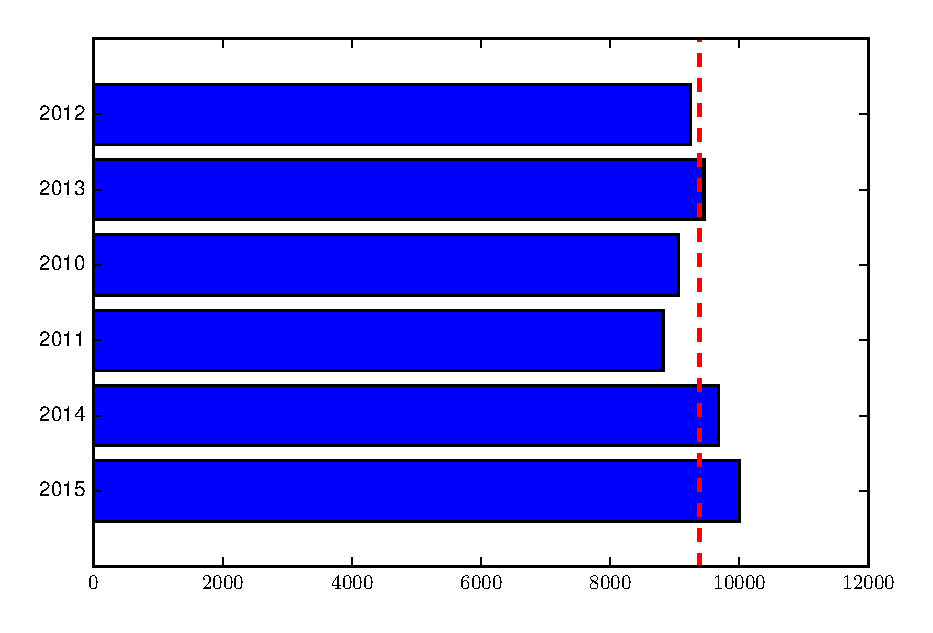
\includegraphics[scale=0.7]{figuras/TotalAccidentsPerAny.eps}
	\caption{Total d'accidents per any}
    \label{fig:totalaccidentsany}
\end{figure}

\subsubsection*{Mapes de calor}

Per fer-nos una idea dels accidents respecte a la seva localització, hem fet mapes de calor, així sabem en quines zones es concentren més accidents i en quines no.

En el mapa de 2010 (figura \ref{fig:heatmap0} pàgina \pageref{fig:heatmap0}) observem que es va concentrar molts accidents per la zona de carrer Aragó amb carrer Balmes, rambla de Catalunya i Passeig de Gràcia. En canvi, en mapes com el del 2011 (figura \ref{fig:heatmap1} pàgina \pageref{fig:heatmap1}) no hi ha tanta concentració en una zona, però hi ha més zones de concentracions d'accidents, com per exemple en aquest cas, hi ha concentracions en Gran Via de les Corts Catalanes, a l'altura d'Universitat i Comte Urgell.

En general sempre s'aprecia grans concentracions d'accidents a zona de l'Eixample, entre Diagonal i Gran Via, i entre carrer de Sants i Passeig de gràcia. Però en mapes com el de 2014 (figura \ref{fig:heatmap4} pàgina \pageref{fig:heatmap4}) i el de 2015 (figura \ref{fig:heatmap5} pàgina \pageref{fig:heatmap5}), també veiem concentracions notables d'accidents per la zona de Clot i de Bogatell.

\subsubsection*{Accidents per districte}

Els numero d'accidents per districte (figura\ref{fig:totaldistricte} i figura \ref{fig:districtes} pàgina \pageref{fig:districtes}) ens fa veure com els d'accidents a l'Eixample (2710 de mitja anual) és el 28\% dels accidents a tota Barcelona. Per darrere venen districtes com Sant Martí, Sarrià-Sant Gervasi i Sants-Montjuïc que contenen un 10\% dels accidents. La resta de districtes ronden el 5\%.

\begin{figure}[H]
\footnotesize
\centering
\stackunder[5pt]{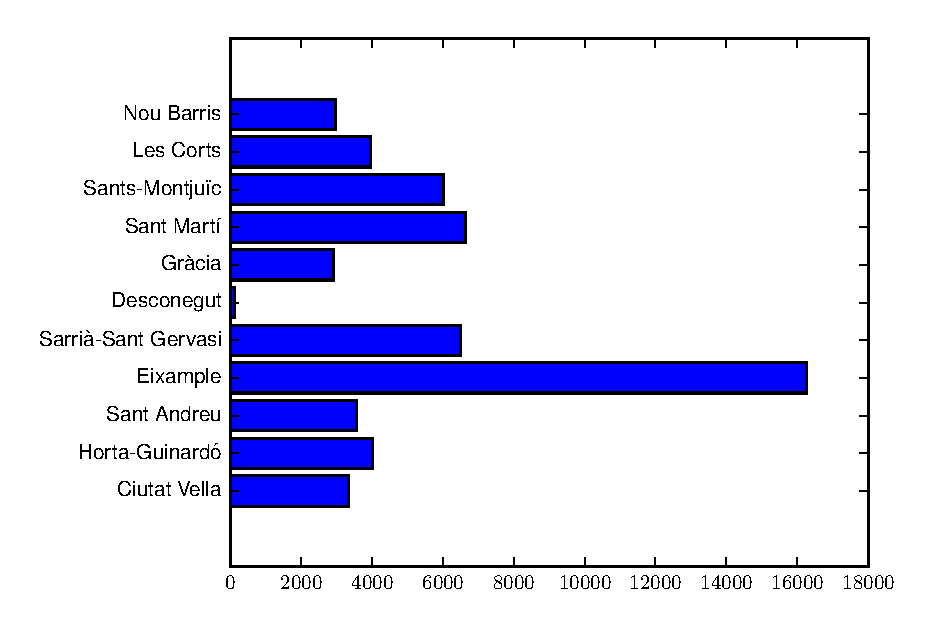
\includegraphics[width=3in]{figuras/NomDistricteTotalsBar.eps}}{Totals 2010-2015}%
%\hspace{1cm}%
\stackunder[5pt]{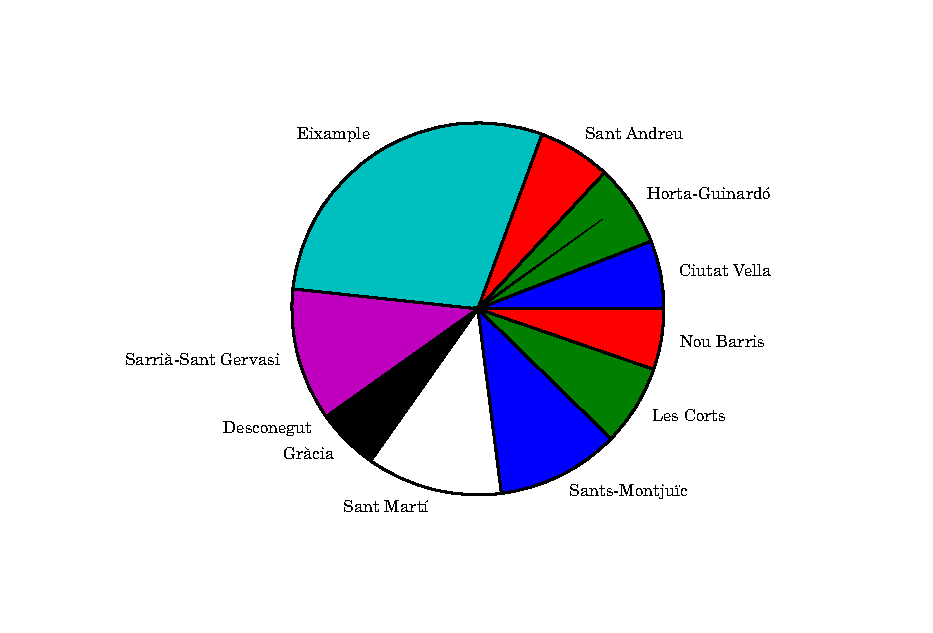
\includegraphics[width=3in]{figuras/NomDistricteMeanPie.eps}}{Mitja}
\caption{Accidents per districte}
\label{fig:totaldistricte}
\end{figure}
\subsubsection*{Accidents per barri}
Respecte als accidents, solament hem mirat els 10 amb més accidents (figura \ref{fig:totalbarri} i figura \ref{fig:barris} pàgina \pageref{fig:barris}), ja que hi ha 73 barris a Barcelona. El barri més destacat és la Dreta de l'Eixample, que té una mitja de 1060 accidents per any, 554 més que el segon, l'Antiga Esquerra de l'Eixample, que té una mitja de 506 accidents per any. Barris per sobre del 300 accidents per any també trobem Sant Gervasi – Galvany (amb 422 accidents per any), la Nova Esquerra de l'Eixample (amb 353 accidents per any) i la Sagrada Família (amb 301 accidents per any). Entre 300 i 200 accidents trobem les Corts, el Fort Pienc, el Poble Sec, Sant Antoni i la Maternitat i Sant Ramon. 

\begin{figure}[H]
\footnotesize
\centering
\stackunder[5pt]{\includegraphics[width=3in]{figuras/NomBarriTopTotalsBar.eps}}{Totals 2010-2015}%
%\hspace{1cm}%
\stackunder[5pt]{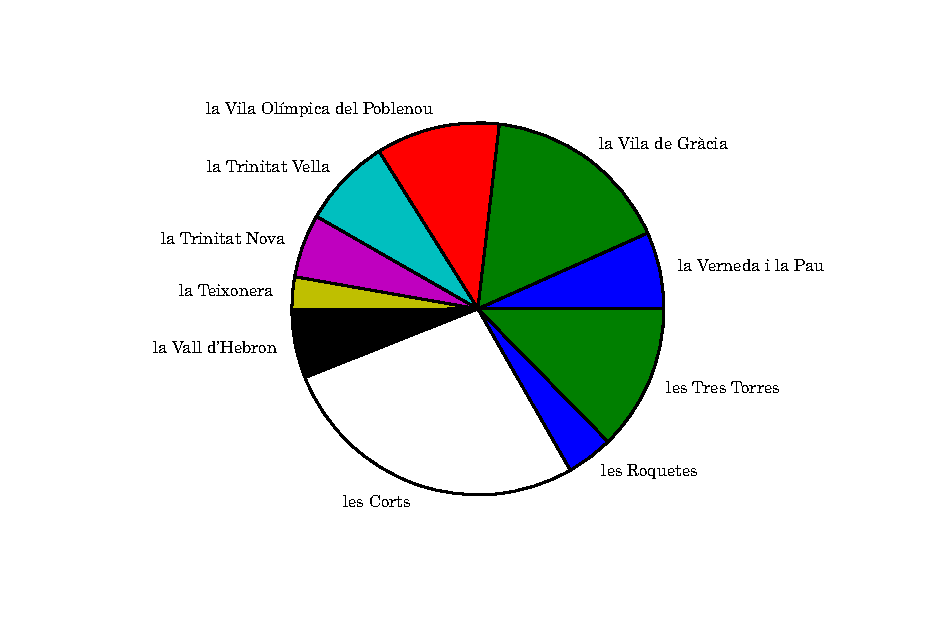
\includegraphics[width=3in]{figuras/NomBarriTopMeanPie.eps}}{Mitja}
\caption{Accidents per barri}
\label{fig:totalbarri}
\end{figure}

\subsubsection*{Accidents per carrer}

En el rànquing d'accidents per carrers (figura \ref{fig:totalcarrer} i figura \ref{fig:carrers} pàgina \pageref{fig:carrers}) veiem que els dos primers són, amb diferència, la Gran Via de les Corts Catalanes, amb una mitja de 471 accidents per any, i Diagonal, amb una mitja de 402 accidents per any. Posteriorment ve Aragó amb 227 accidents l'any. La resta de carrers ja tenen una mitja d'accidents inferior a 200, com per exemple, Litoral (Llobregat) amb 172 o Meridiana amb 166.

\begin{figure}[H]
\footnotesize
\centering
\stackunder[5pt]{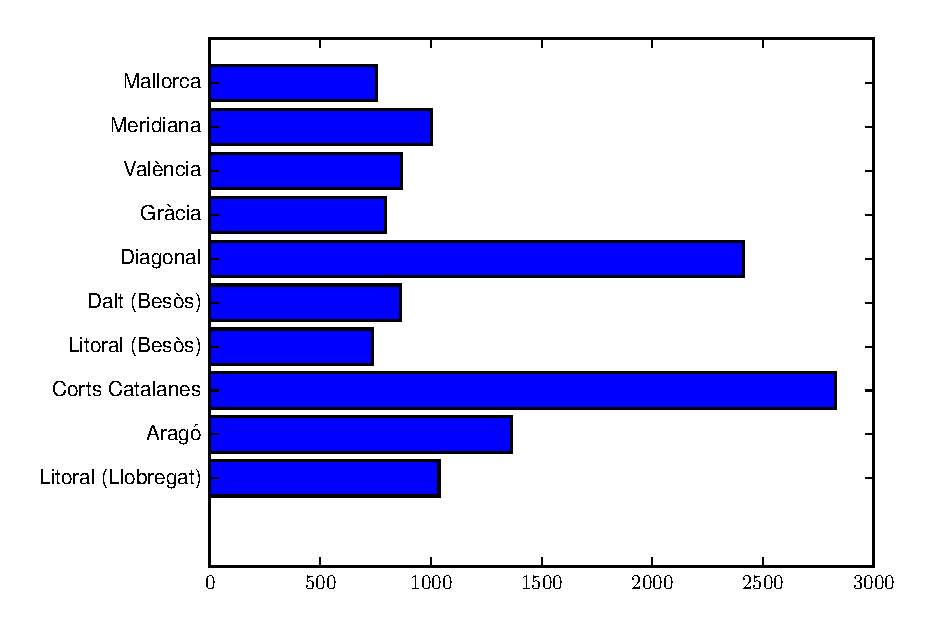
\includegraphics[width=3in]{figuras/NomCarrerTopTotalsBar.eps}}{Totals 2010-2015}%
%\hspace{1cm}%
\stackunder[5pt]{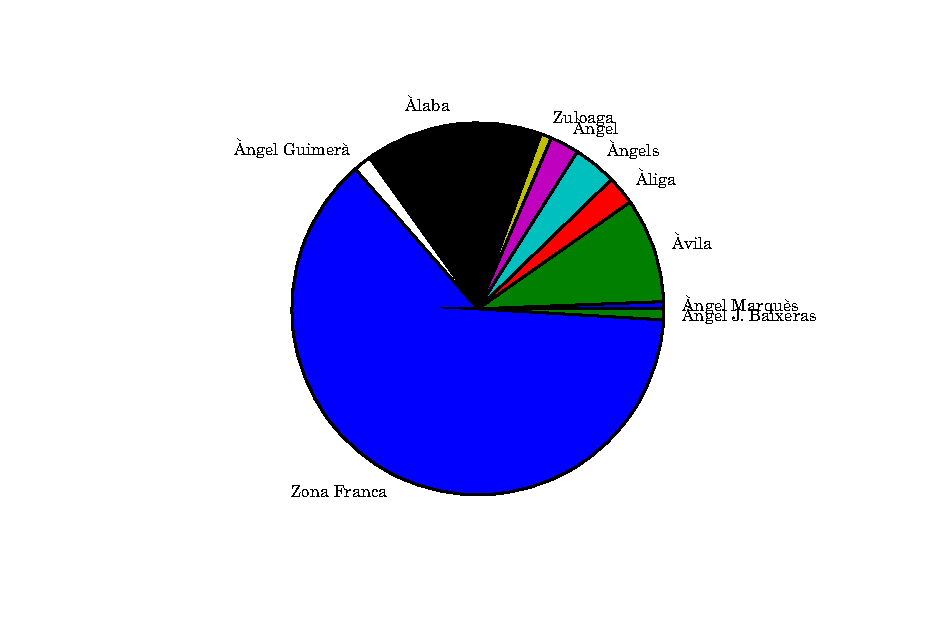
\includegraphics[width=3in]{figuras/NomCarrerTopMeanPie.eps}}{Mitja}
\caption{Accidents per carrer}
\label{fig:totalcarrer}
\end{figure}

\subsubsection*{Accidents per mes}

Quan mirem els accidents per mes (figura \ref{fig:totalmes} i figura \ref{fig:mesplot} pàgina \pageref{fig:mesplot}) de l'any, veiem que sembla que a la tardor hi ha més accidents, ja que l'Octubre i el Novembre són els dos mesos amb més accidents (amb 837 i 835 accidents de mitja respectivament). Entre el mes amb més accidents (Octubre amb 837) i el penúltim (Gener amb 743) hi ha solament una diferència de quasi 100 accidents, en canvi, la diferència entre el penúltim i Agost (l'últim amb 576) hi ha una diferència de 167 accidents.

\begin{figure}[H]
\footnotesize
\centering
\stackunder[5pt]{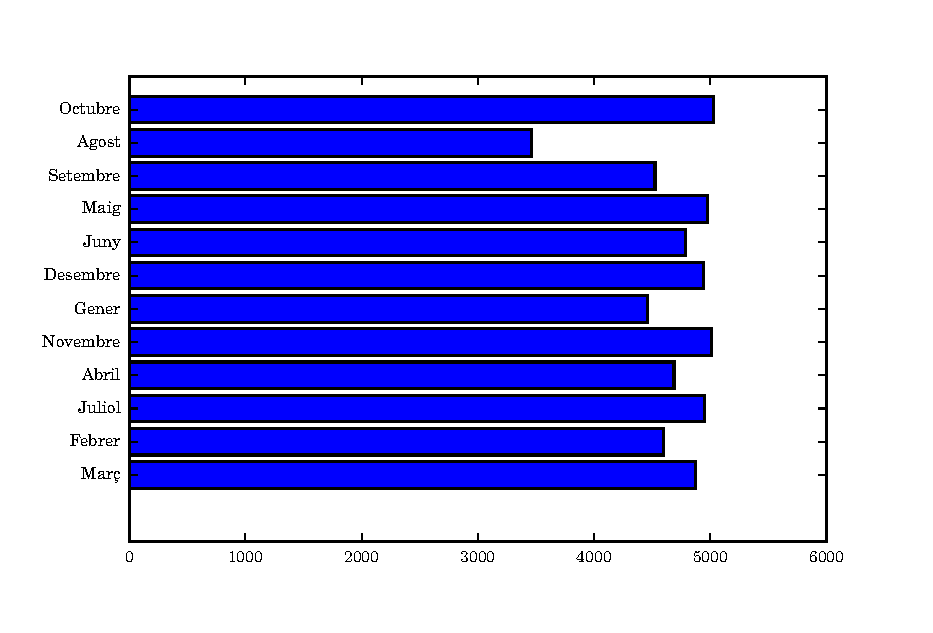
\includegraphics[width=3in]{figuras/NomMesTotalsBar.eps}}{Totals 2010-2015}%
%\hspace{1cm}%
\stackunder[5pt]{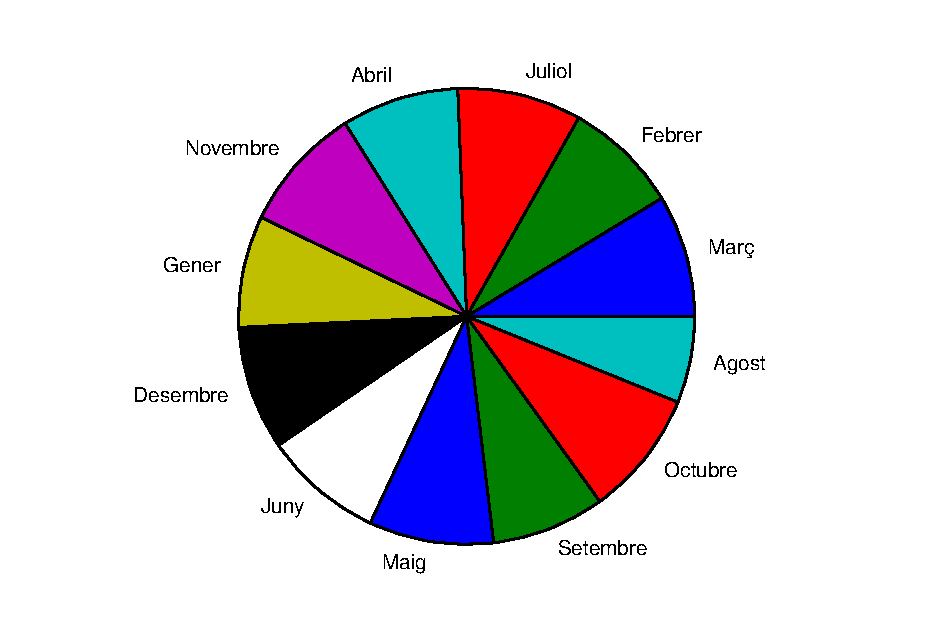
\includegraphics[width=3in]{figuras/NomMesMeanPie.eps}}{Mitja}
\caption{Accidents per mes}
\label{fig:totalmes}
\end{figure}

\subsubsection*{Accidents per dia de la setmana}

Estudiant els accidents pels dies de la setmana (figura \ref{fig:totalsetmana} i figura \ref{fig:setmana} pàgina \pageref{fig:setmana}), veiem que el dia de la setmana amb més accidents de trànsit és el divendres amb una mitja de 1632. En canvi el dia de la setmana laboral amb menys accidents el dilluns amb 1423. De mitja durant la setmana laboral hi ha una mitja 1519 accidents, però durant el cap de setmana baixen els números. El dissabte amb una mitja de 1010 i el diumenge (el dia de la setmana amb menys accidents) amb 771 accidents de mitja.

\begin{figure}[H]
\footnotesize
\centering
\stackunder[5pt]{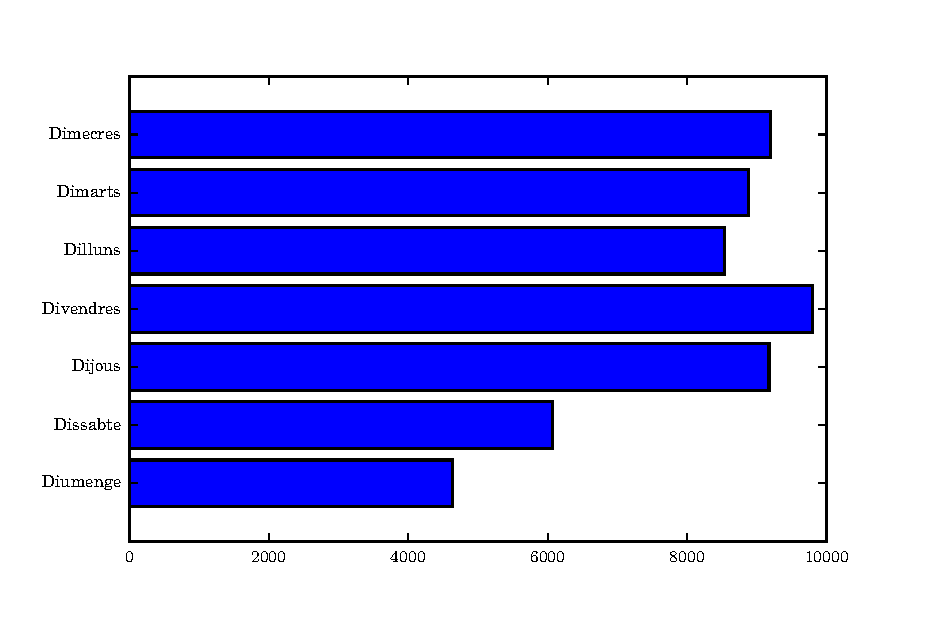
\includegraphics[width=3in]{figuras/DescripcioDiaSetmanaTotalsBar.eps}}{Totals 2010-2015}%
%\hspace{1cm}%
\stackunder[5pt]{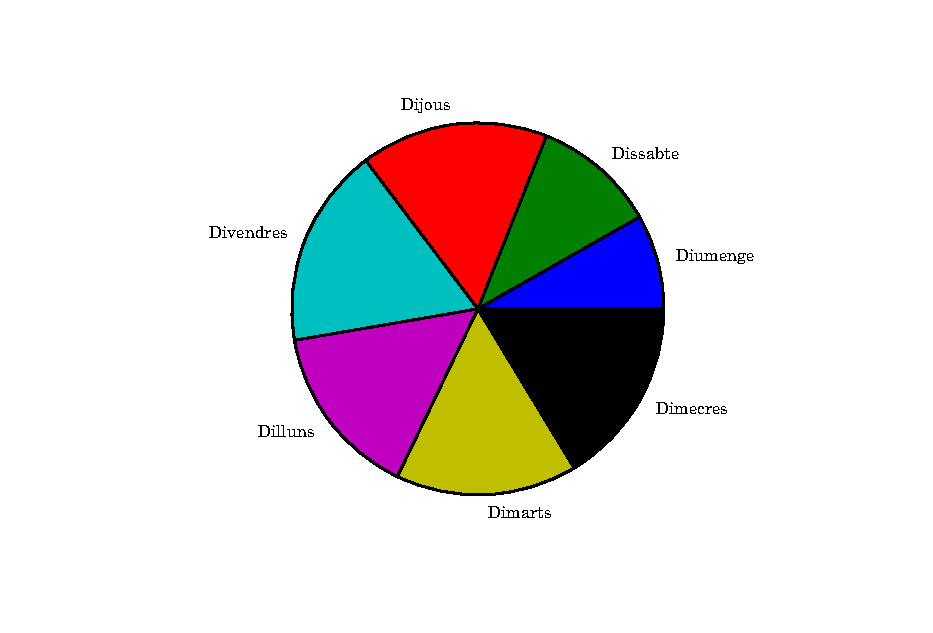
\includegraphics[width=3in]{figuras/DescripcioDiaSetmanaMeanPie.eps}}{Mitja}
\caption{Accidents per dia de la setmana}
\label{fig:totalsetmana}
\end{figure}

\subsubsection*{Accidents per TODO}
%TODO Accidents per persones

\subsection{Conclusió de l'exploració}
Després de l'estudi geogràfic que hem fet, podem corrobora part del que hem vist inicialment al mapa. Com ben havíem avançat al mapa de calor, els accidents principalment es concentren en la zona de l'eixample, dividits entre Aragó i Gran via de les Corts Catalanes, dos dels carrers més transitats de Barcelona. A banda d'aquestes també trobem el Carrer Diagonal, que és justificable el seu nombre d'accidents, ja que és l'arteria principal del tràfic de la ciutat.

En qüestió temporal ens atrevim a afirmar que els dies no lectius i més els dies laborals, fan que descendeixi els accidents. El cap de setmanes descendeixen molt els accidents com també mesos com Agost. Per algun fet, també hi ha més accidents el divendres que els dilluns, això podria estar degut a l'actitud de la gent en aquests dos dies. Un altre punt curiós és que a la tardor hi ha més accidents, sobretot a l'Octubre i al Novembre.



\newpage
\section{Anàlisi exhaustiu}

\subsection{Plantejament de les hipotesis}

\subsection{Enrequiment de les dades}



\subsection{Anàlisis}

\subsection{Presentació de resultats}


\newpage
\section{Conclusió i treball futur}

\subsection{Conclusió}

\subsection{Treball futur}



\newpage
\section{Bibliografia}

\newpage
\section{Anexos}
\subsection*{Mapes}
\begin{sidewaysfigure}[ht]
    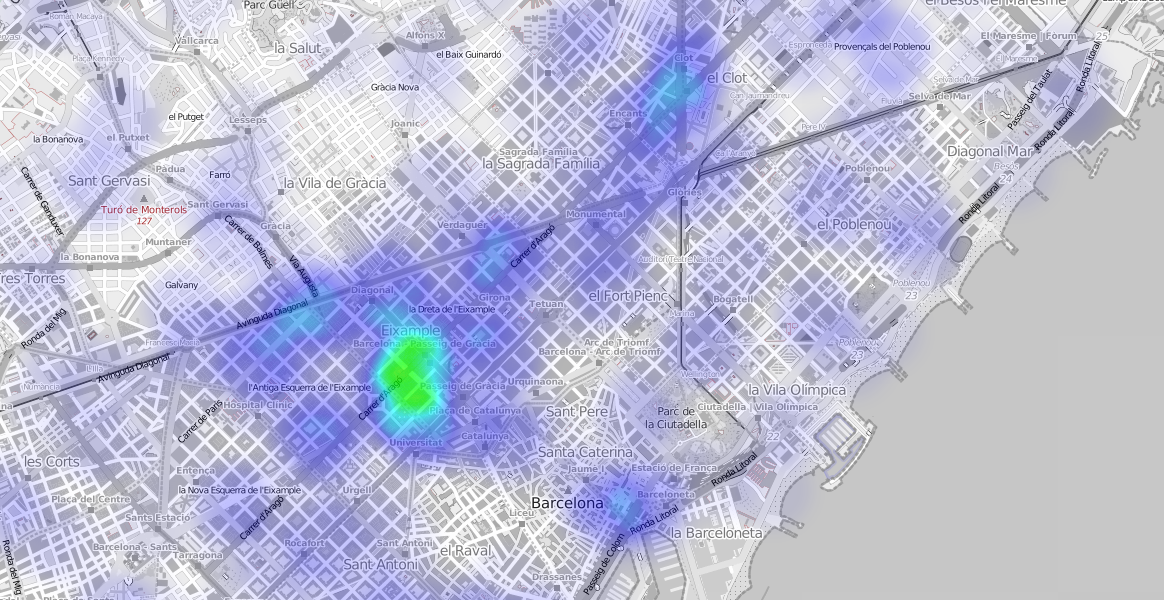
\includegraphics[width=\textwidth,height=\textheight,keepaspectratio]{mapesImg/heatmap2010.png}
    \caption{Mapa de calor 2010}
    \label{fig:heatmap0}
\end{sidewaysfigure}
\begin{sidewaysfigure}[ht]
    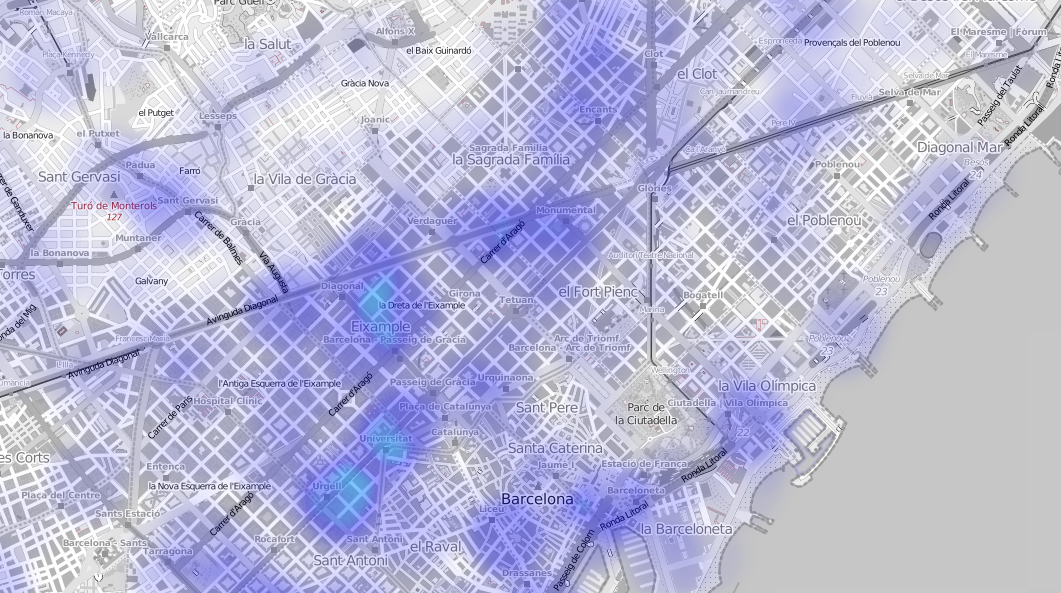
\includegraphics[width=\textwidth,height=\textheight,keepaspectratio]{mapesImg/heatmap2011.png}
    \caption{Mapa de calor 2011}
    \label{fig:heatmap1}
\end{sidewaysfigure}

\begin{sidewaysfigure}[ht]
    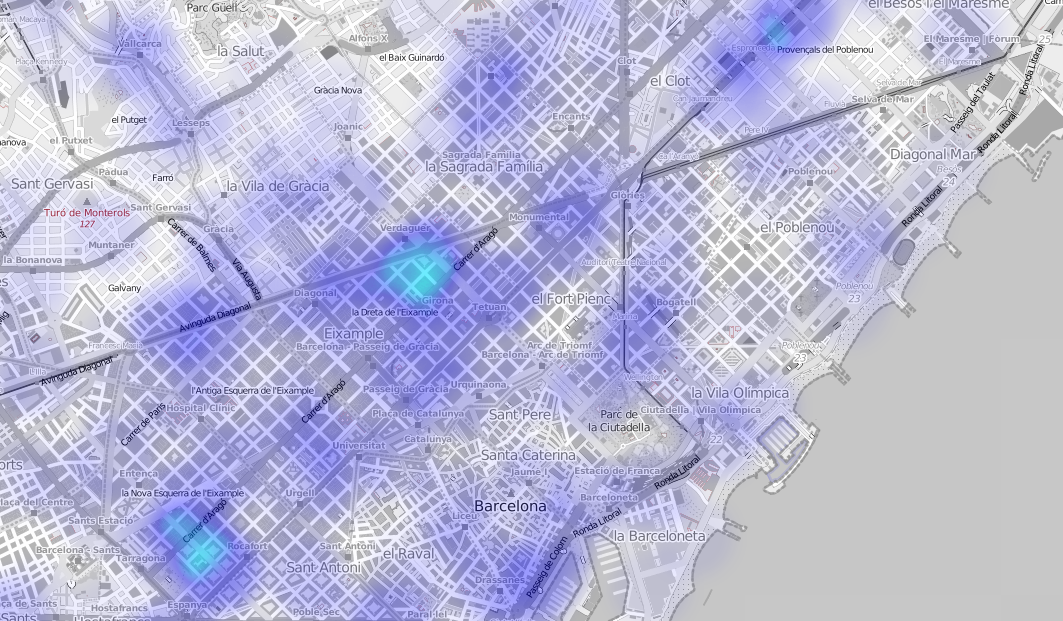
\includegraphics[width=\textwidth,height=\textheight,keepaspectratio]{mapesImg/heatmap2012.png}
    \caption{Mapa de calor 2012}
    \label{fig:heatmap2}
\end{sidewaysfigure}

\begin{sidewaysfigure}[ht]
    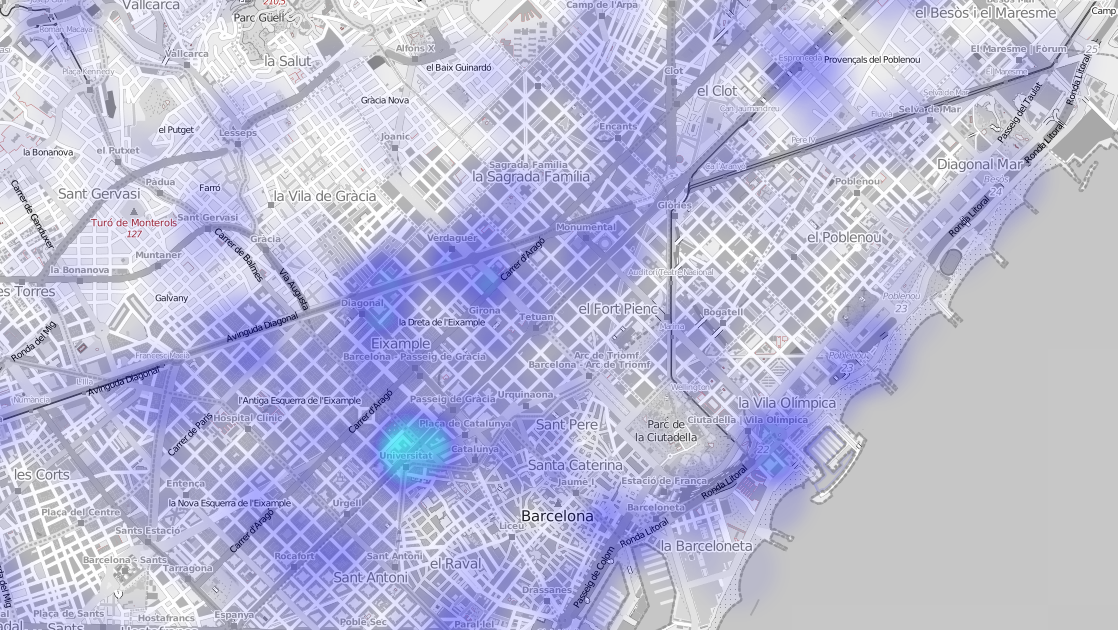
\includegraphics[width=\textwidth,height=\textheight,keepaspectratio]{mapesImg/heatmap2013.png}
    \caption{Mapa de calor 2013}
    \label{fig:heatmap3}
\end{sidewaysfigure}

\begin{sidewaysfigure}[ht]
    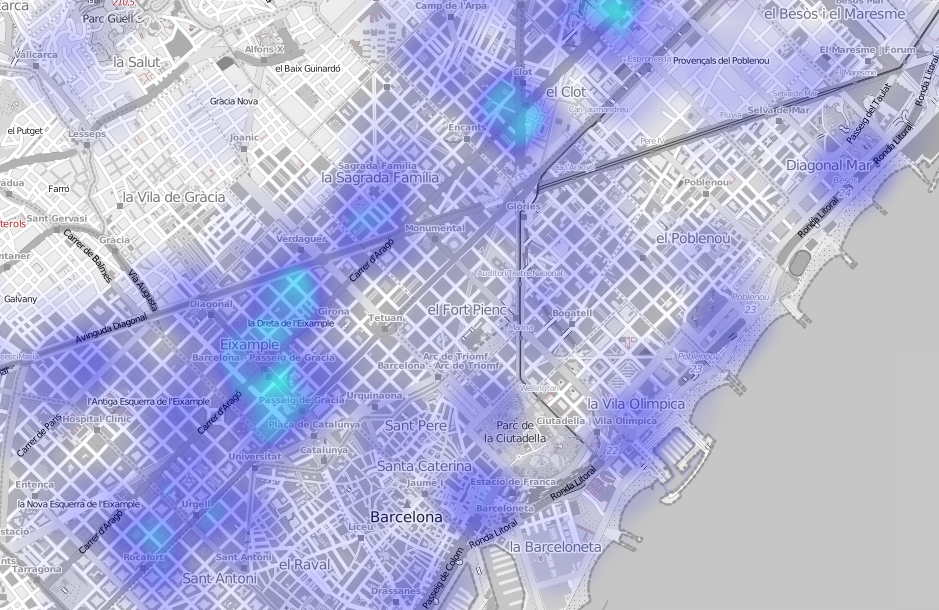
\includegraphics[width=\textwidth,height=\textheight,keepaspectratio]{mapesImg/heatmap2014.png}
    \caption{Mapa de calor 2014}
    \label{fig:heatmap4}
\end{sidewaysfigure}
\begin{sidewaysfigure}[ht]
    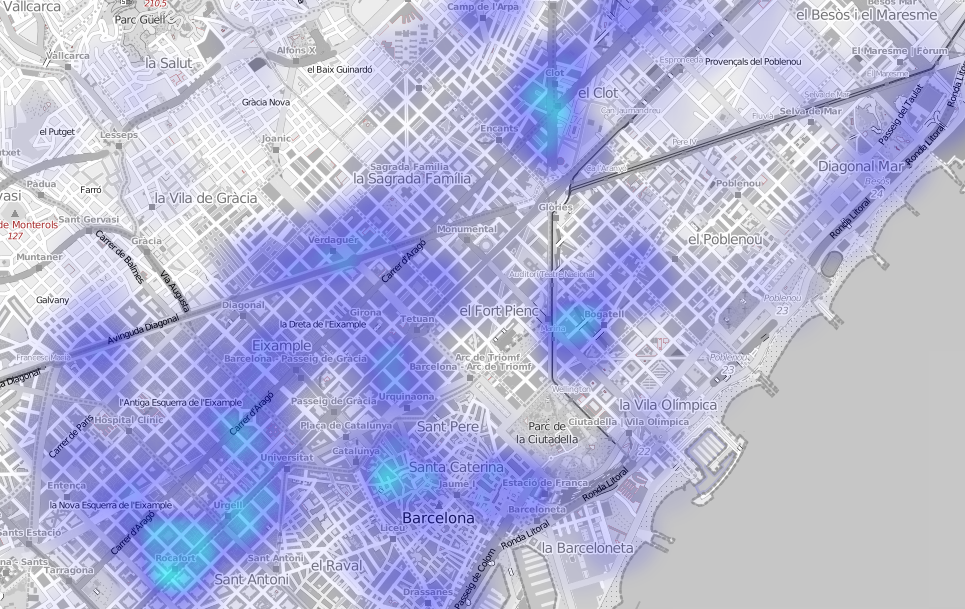
\includegraphics[width=\textwidth,height=\textheight,keepaspectratio]{mapesImg/heatmap2015.png}
    \caption{Mapa de calor 2015}
    \label{fig:heatmap5}
\end{sidewaysfigure}


\newpage
\subsection*{Plots}

\begin{figure}
\begin{tabular}{cc}
\subfloat[2010]{\includegraphics[width = 3in]{figuras/NomDistricte2010.eps}} &
\subfloat[2011]{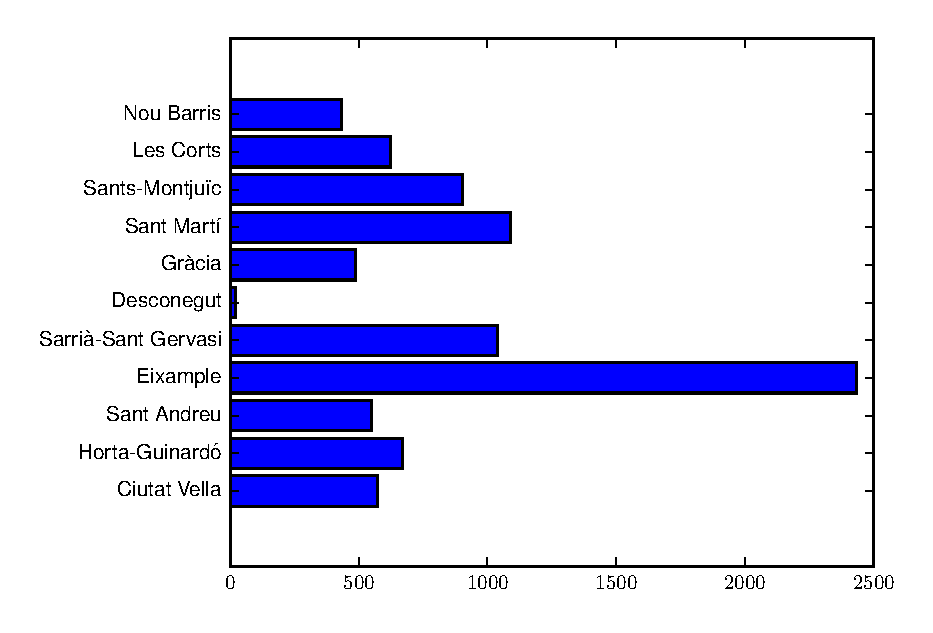
\includegraphics[width = 3in]{figuras/NomDistricte2011.eps} }\\
\subfloat[2012]{\includegraphics[width = 3in]{figuras/NomDistricte2012.eps} } &
\subfloat[2013]{\includegraphics[width = 3in]{figuras/NomDistricte2013.eps}}\\
\subfloat[2014]{\includegraphics[width = 3in]{figuras/NomDistricte2014.eps}} &
\subfloat[2015]{\includegraphics[width = 3in]{figuras/NomDistricte2015.eps}}
\end{tabular}
\caption{Accidents per Districtes}
\label{fig:districtes}
\end{figure}


\begin{figure}
\begin{tabular}{cc}
\subfloat[2010]{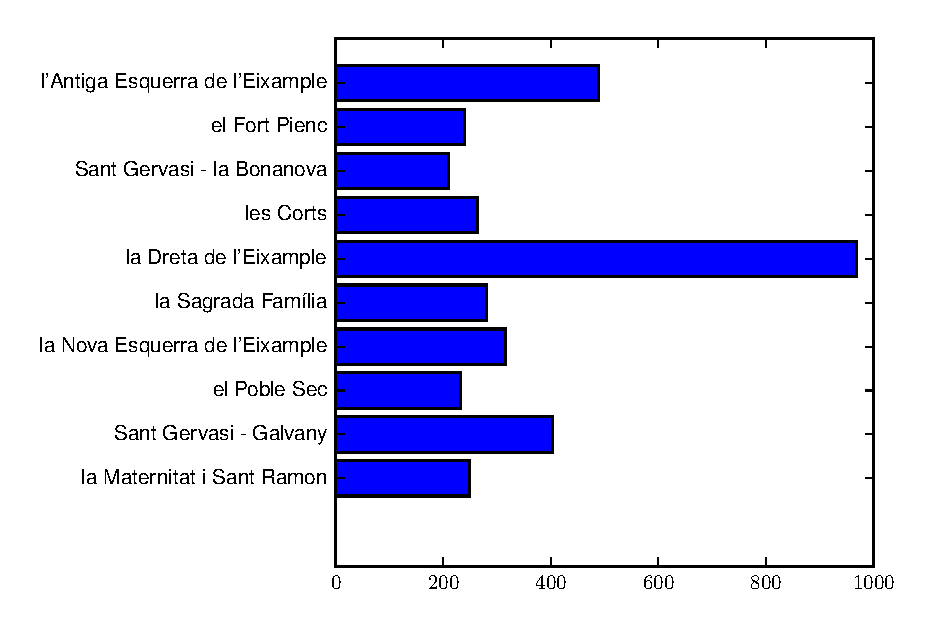
\includegraphics[width = 3in]{figuras/NomBarriTop2010.eps}} &
\subfloat[2011]{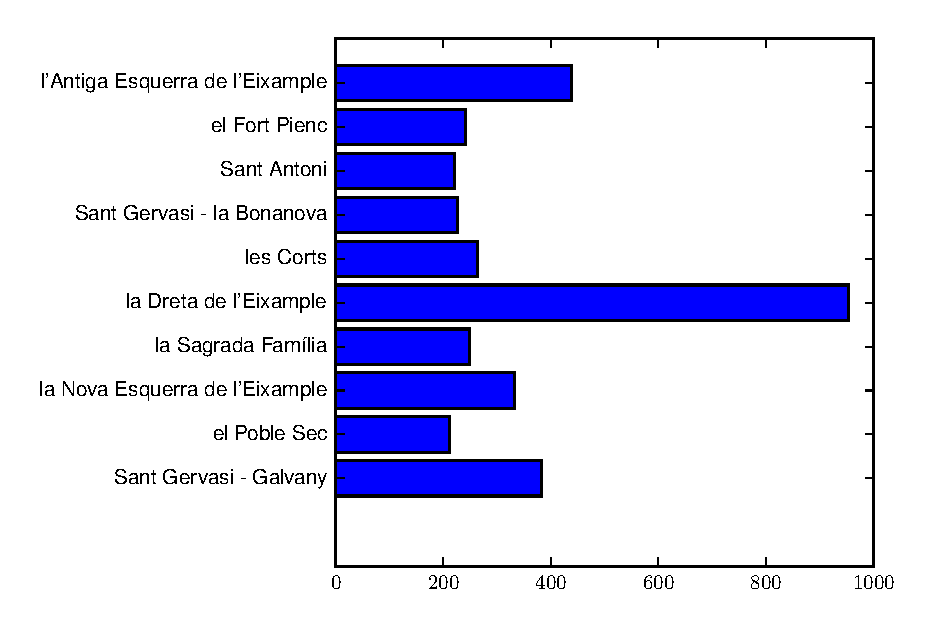
\includegraphics[width = 3in]{figuras/NomBarriTop2011.eps} }\\
\subfloat[2012]{\includegraphics[width = 3in]{figuras/NomBarriTop2012.eps} } &
\subfloat[2013]{\includegraphics[width = 3in]{figuras/NomBarriTop2013.eps}}\\
\subfloat[2014]{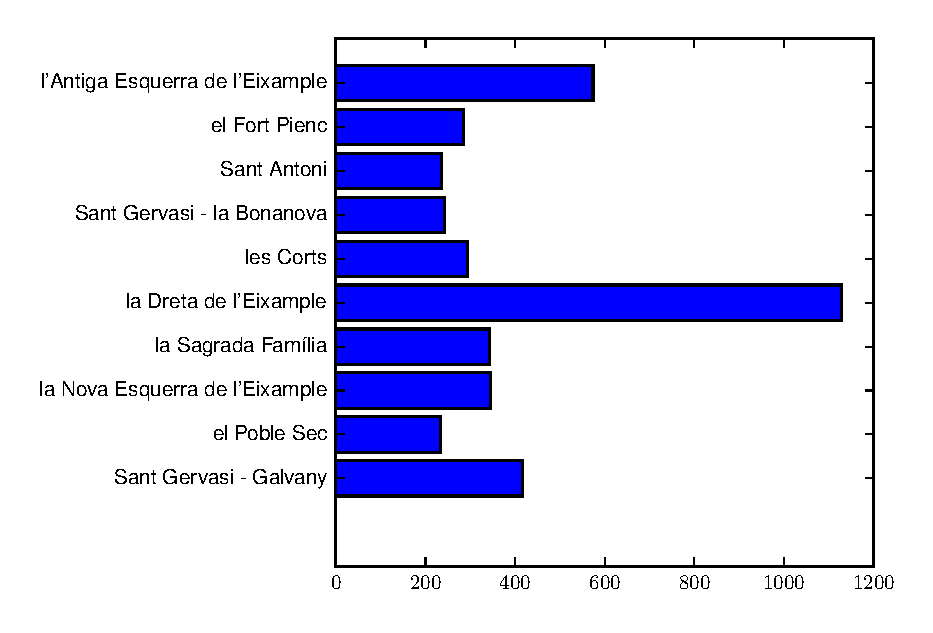
\includegraphics[width = 3in]{figuras/NomBarriTop2014.eps}} &
\subfloat[2015]{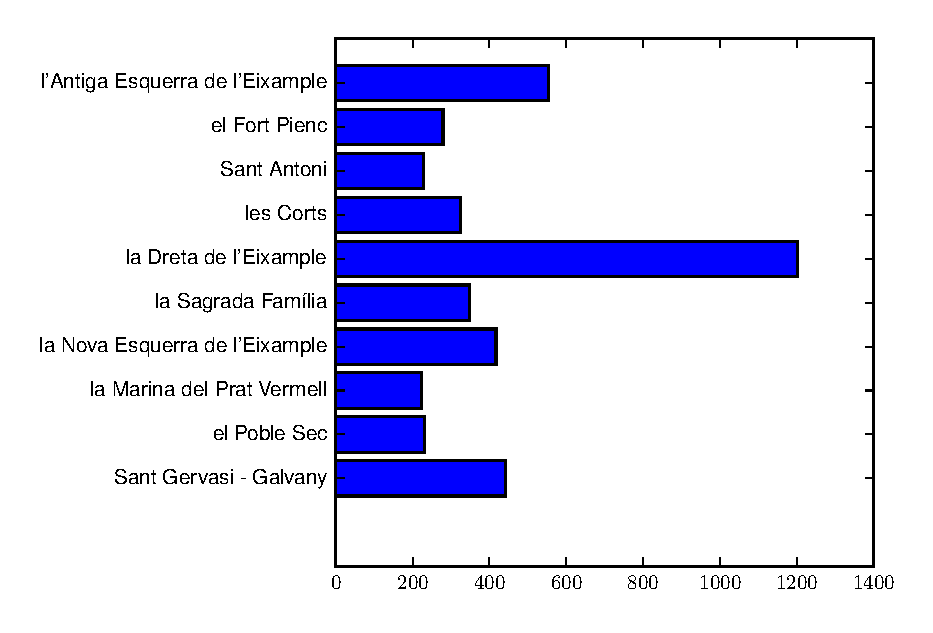
\includegraphics[width = 3in]{figuras/NomBarriTop2015.eps}}
\end{tabular}
\caption{Accidents per Barris}
\label{fig:barris}
\end{figure}

\begin{figure}
\begin{tabular}{cc}
\subfloat[2010]{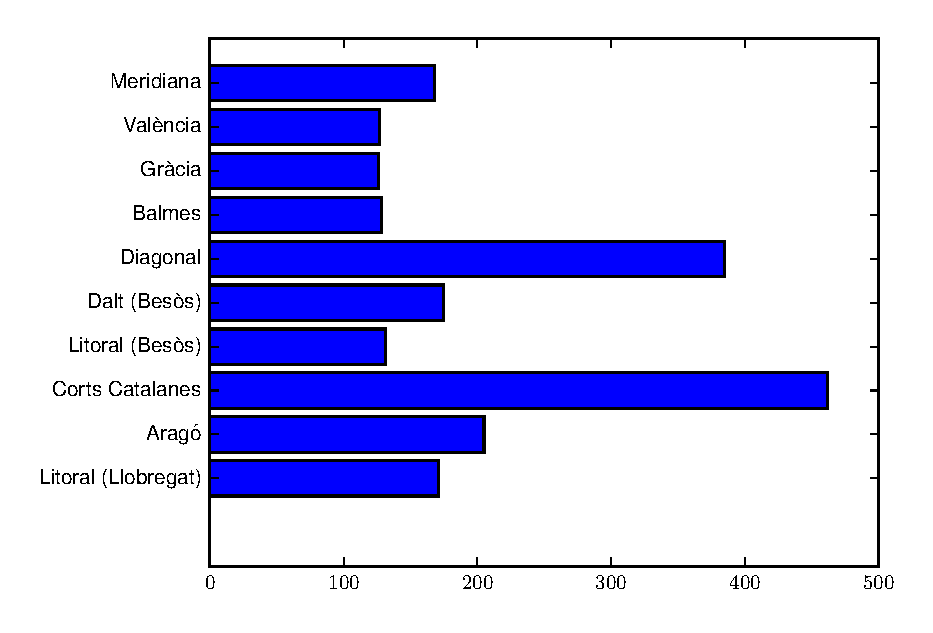
\includegraphics[width = 3in]{figuras/NomCarrerTop2010.eps}} &
\subfloat[2011]{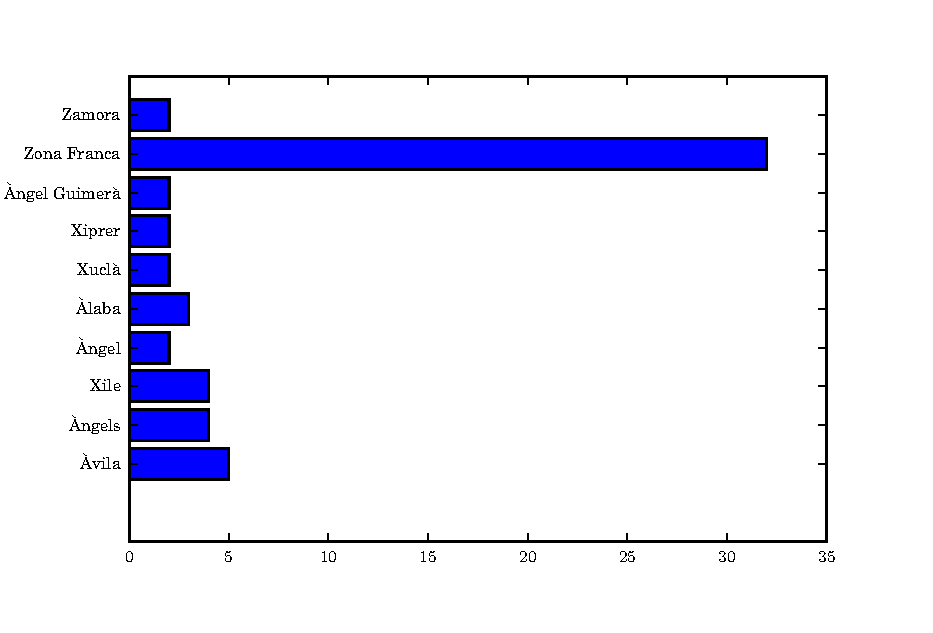
\includegraphics[width = 3in]{figuras/NomCarrerTop2011.eps} }\\
\subfloat[2012]{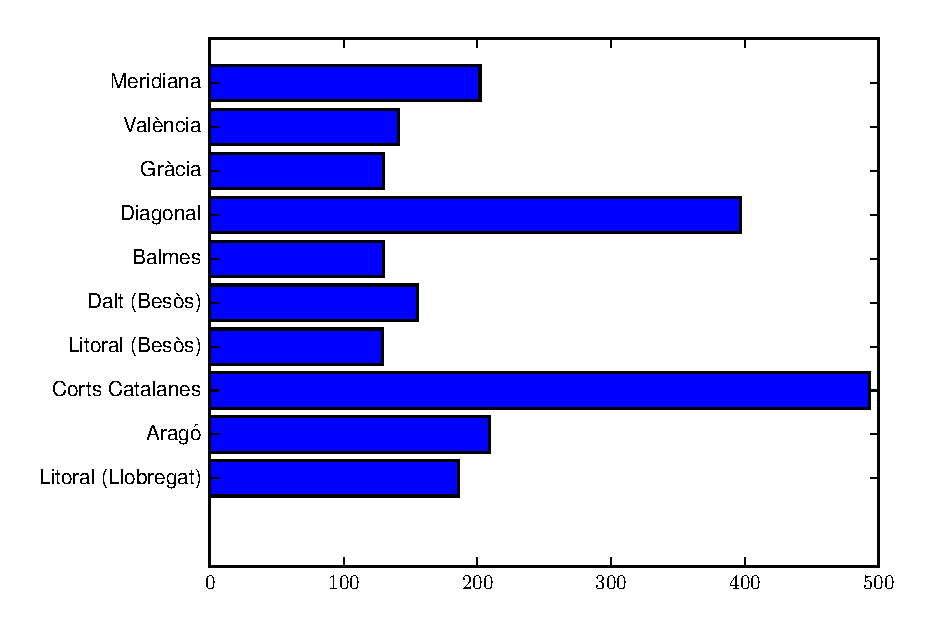
\includegraphics[width = 3in]{figuras/NomCarrerTop2012.eps} } &
\subfloat[2013]{\includegraphics[width = 3in]{figuras/NomCarrerTop2013.eps}}\\
\subfloat[2014]{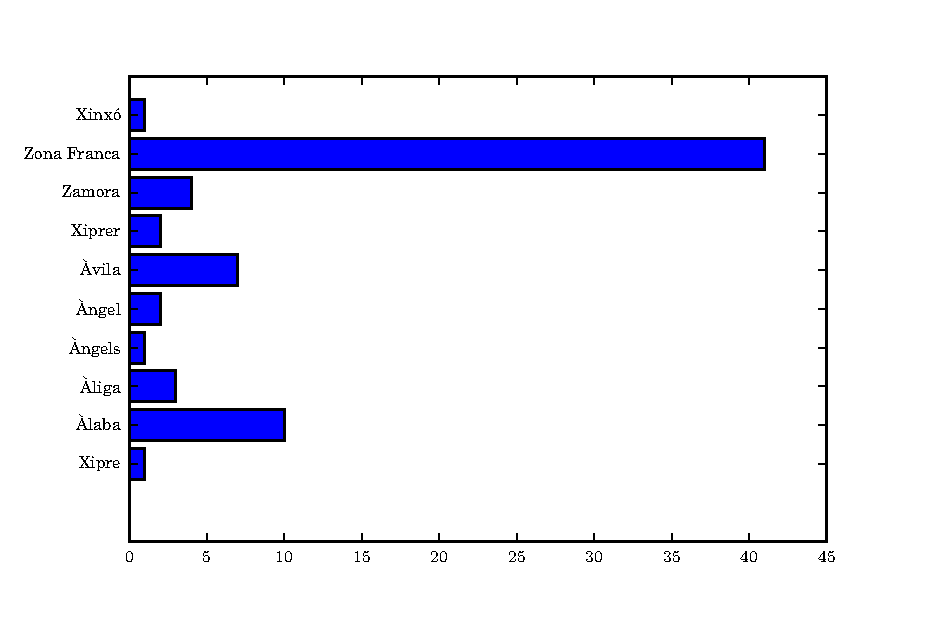
\includegraphics[width = 3in]{figuras/NomCarrerTop2014.eps}} &
\subfloat[2015]{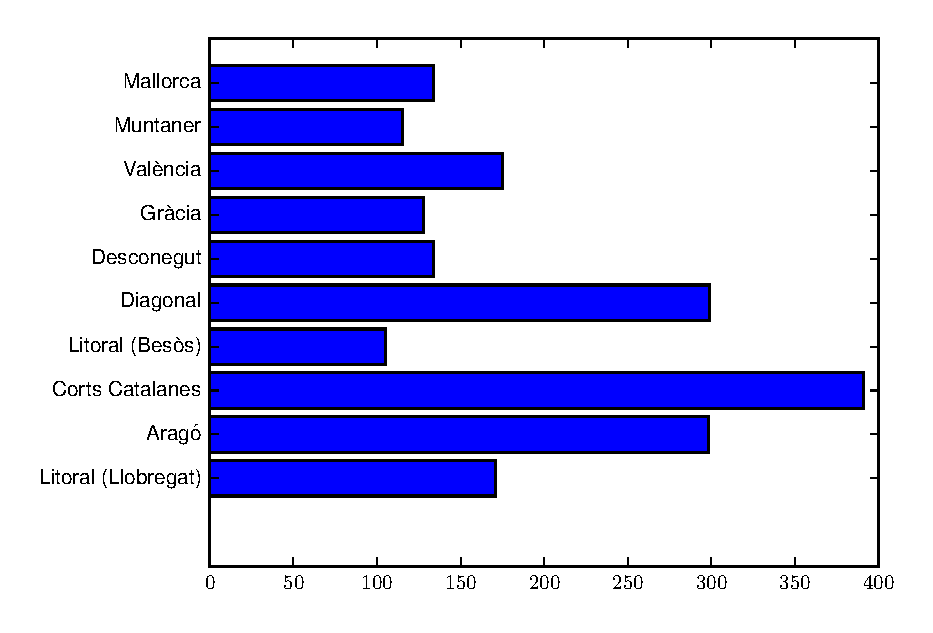
\includegraphics[width = 3in]{figuras/NomCarrerTop2015.eps}}
\end{tabular}
\caption{Accidents per Carrers}
\label{fig:carrers}
\end{figure}

\begin{figure}
\begin{tabular}{cc}
\subfloat[2010]{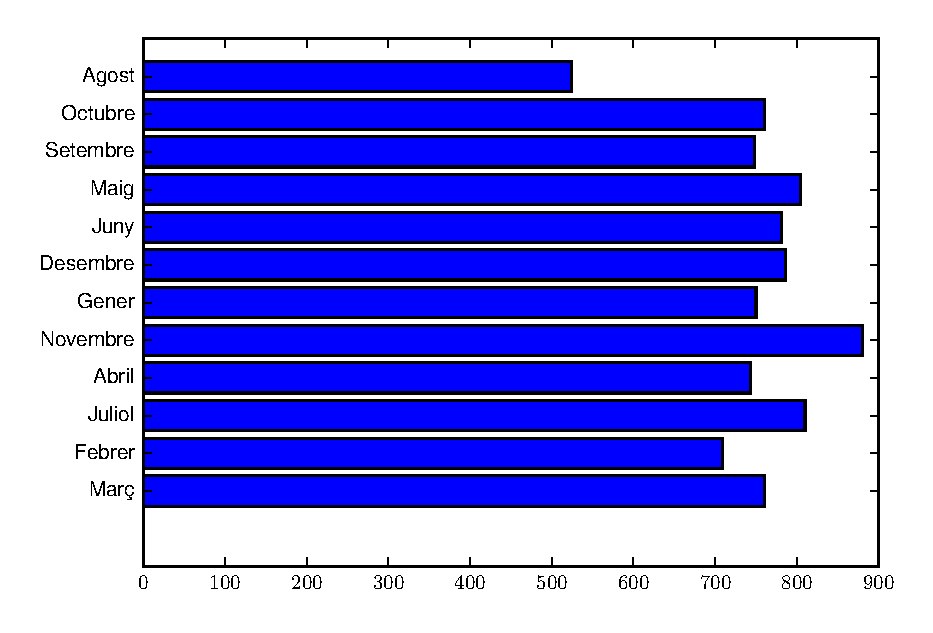
\includegraphics[width = 3in]{figuras/NomMes2010.eps}} &
\subfloat[2011]{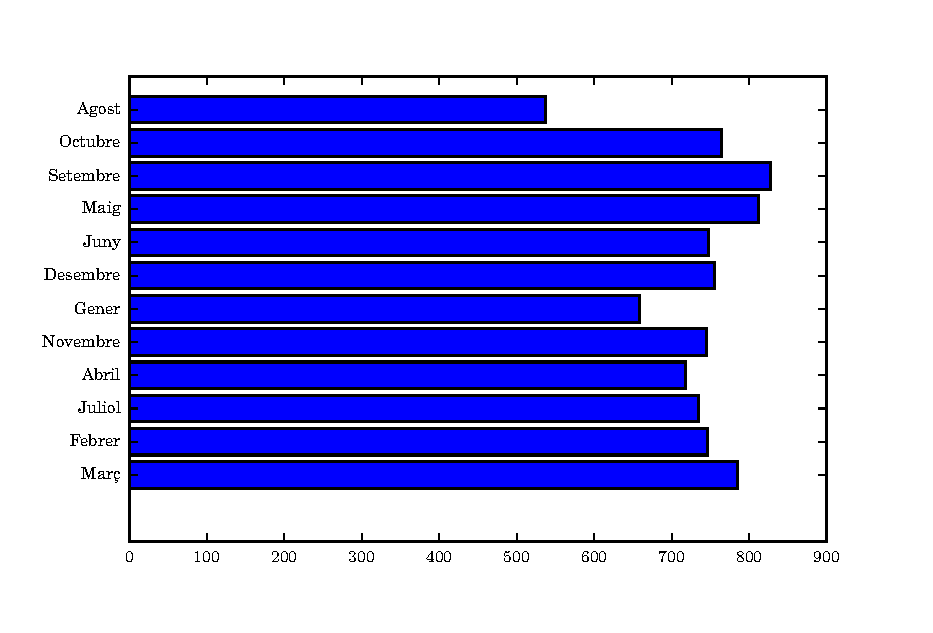
\includegraphics[width = 3in]{figuras/NomMes2011.eps} }\\
\subfloat[2012]{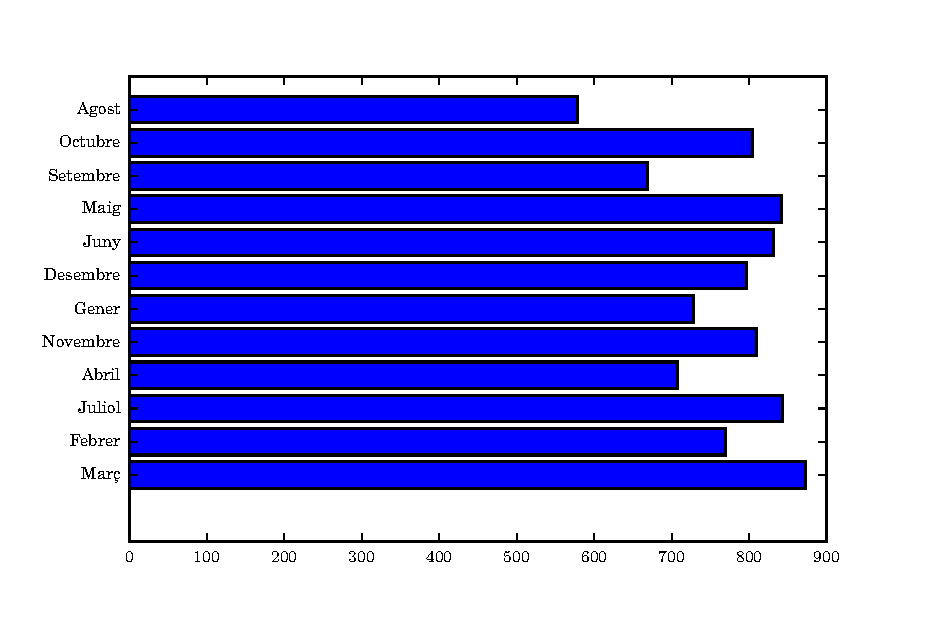
\includegraphics[width = 3in]{figuras/NomMes2012.eps} } &
\subfloat[2013]{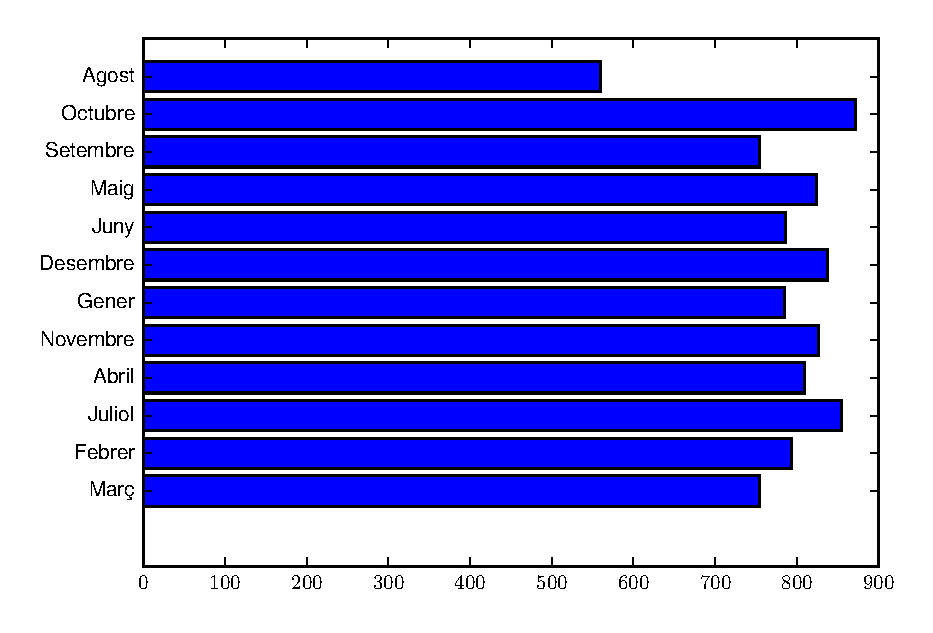
\includegraphics[width = 3in]{figuras/NomMes2013.eps}}\\
\subfloat[2014]{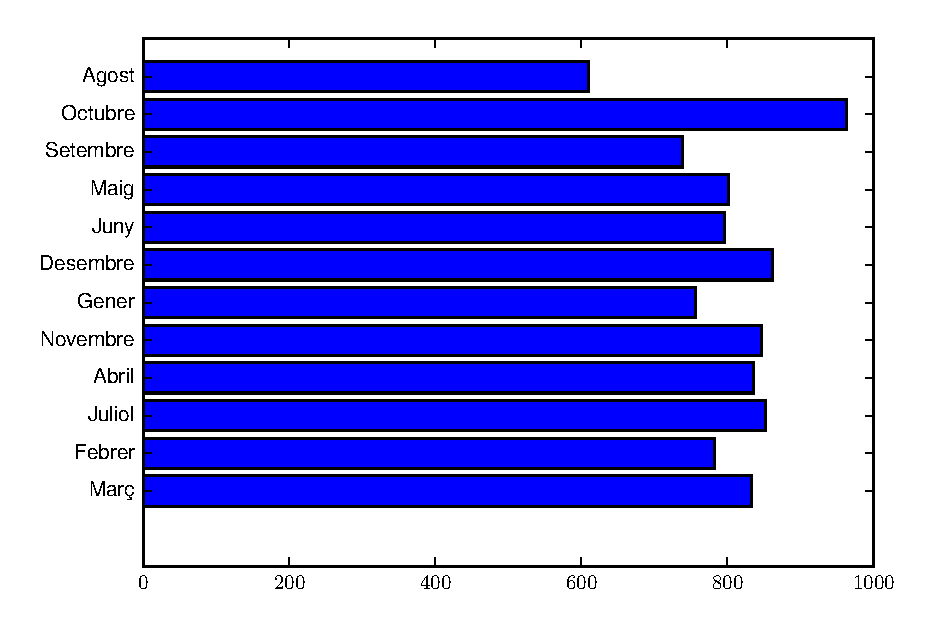
\includegraphics[width = 3in]{figuras/NomMes2014.eps}} &
\subfloat[2015]{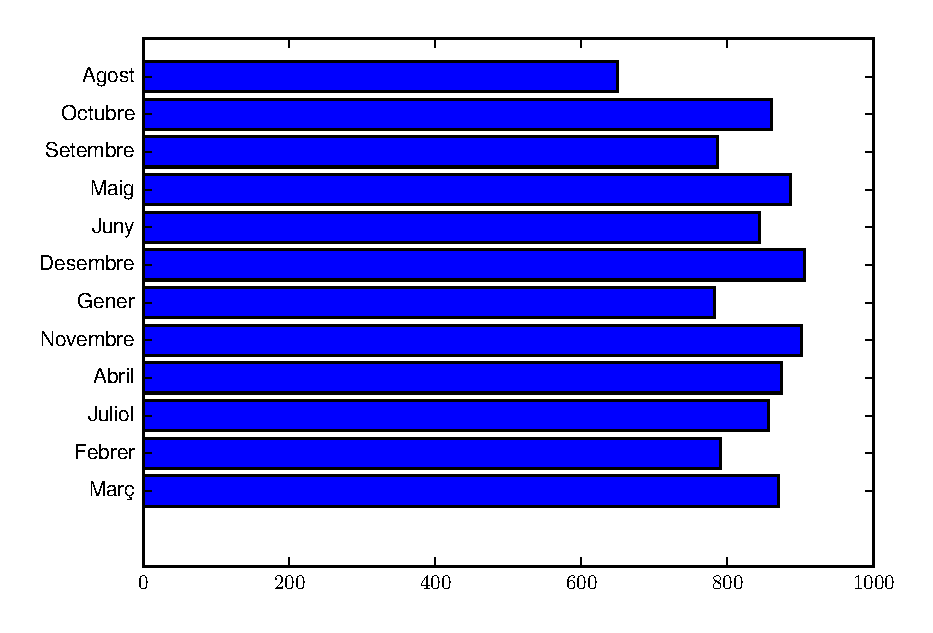
\includegraphics[width = 3in]{figuras/NomMes2015.eps}}
\end{tabular}
\caption{Accidents per mes}
\label{fig:mesplot}
\end{figure}

\begin{figure}
\begin{tabular}{cc}
\subfloat[2010]{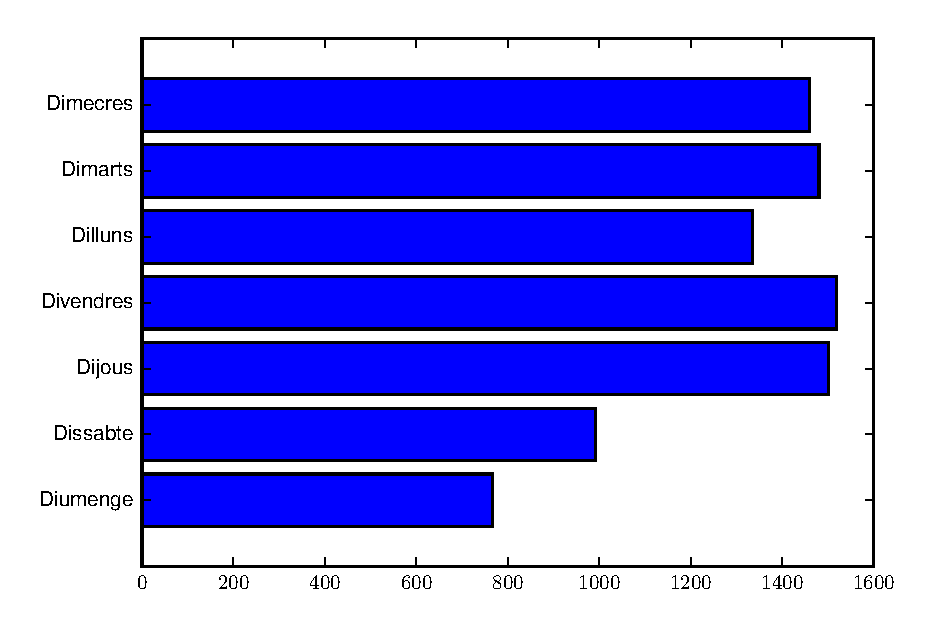
\includegraphics[width = 3in]{figuras/DescripcioDiaSetmana2010.eps}} &
\subfloat[2011]{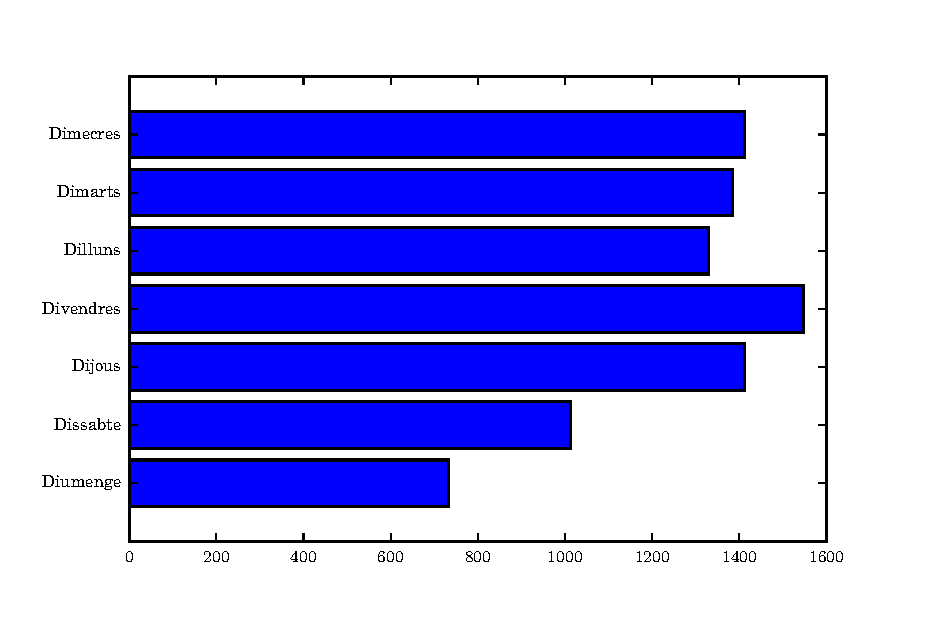
\includegraphics[width = 3in]{figuras/DescripcioDiaSetmana2011.eps} }\\
\subfloat[2012]{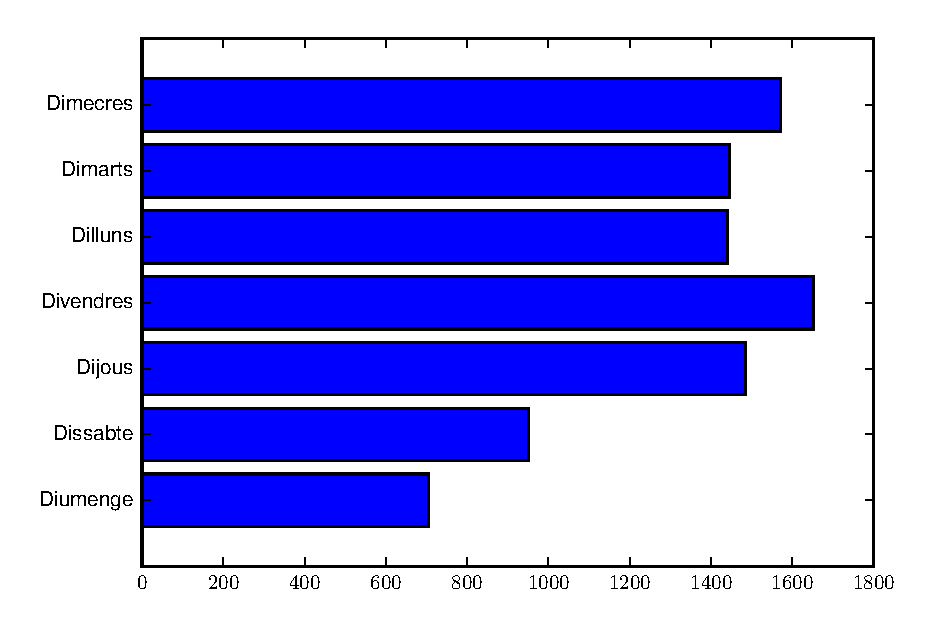
\includegraphics[width = 3in]{figuras/DescripcioDiaSetmana2012.eps} } &
\subfloat[2013]{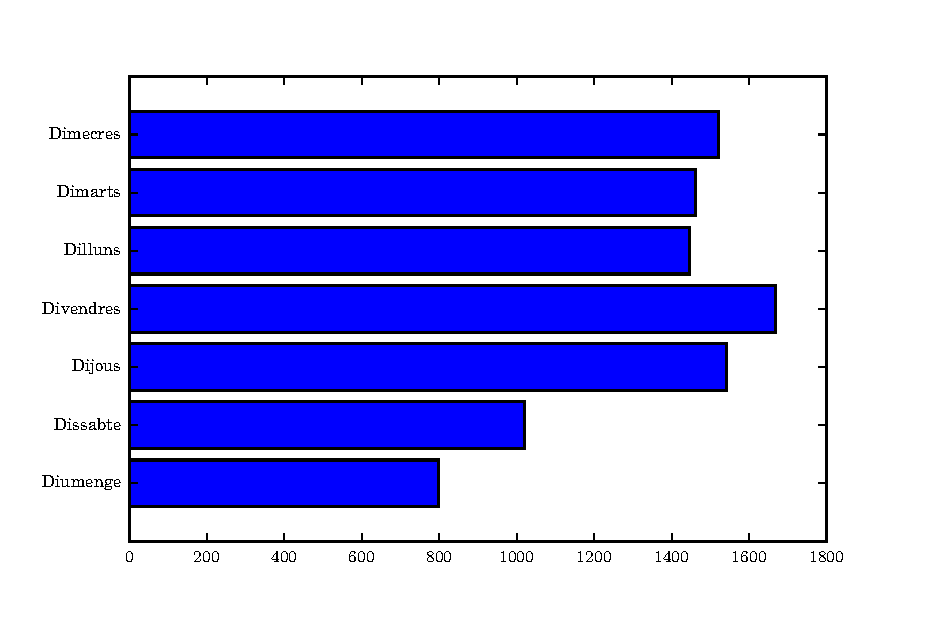
\includegraphics[width = 3in]{figuras/DescripcioDiaSetmana2013.eps}}\\
\subfloat[2014]{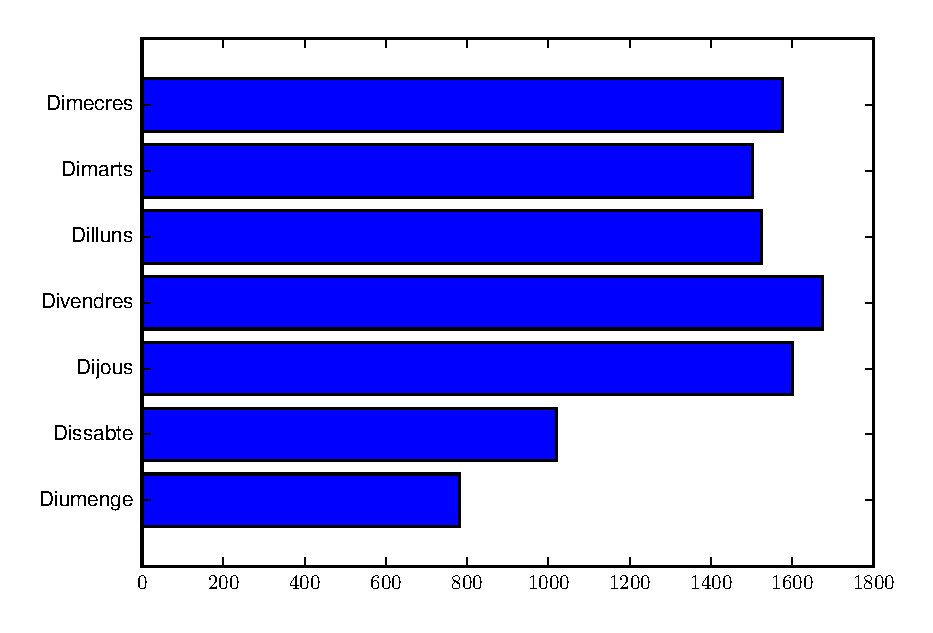
\includegraphics[width = 3in]{figuras/DescripcioDiaSetmana2014.eps}} &
\subfloat[2015]{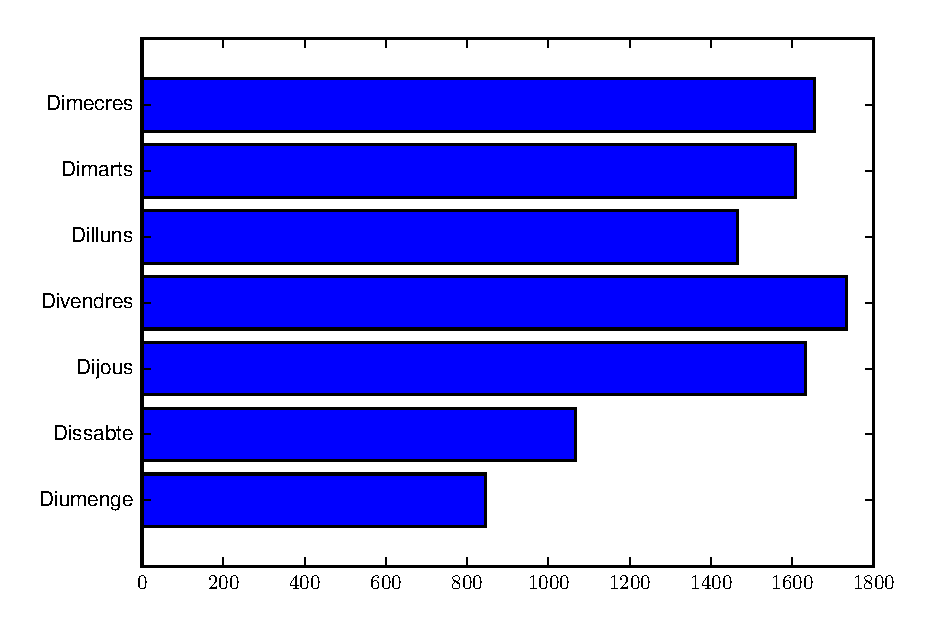
\includegraphics[width = 3in]{figuras/DescripcioDiaSetmana2015.eps}}
\end{tabular}
\caption{Accidents per Setmanes}
\label{fig:setmana}
\end{figure}

%Test antes de añadir la iluminación.
%\begin{figure}[H]
%\centering
%\includegraphics[scale=0.4]{inicialgrafics.png}
%\caption{Sin iluminación.}\label{visina8}
%\end{figure}






\end{document}